\documentclass[tikz,border=5]{standalone}

\usepackage{mathdots}

\usetikzlibrary{calc}
\usetikzlibrary{decorations.pathreplacing}
\usetikzlibrary{scopes}

\begin{document}
  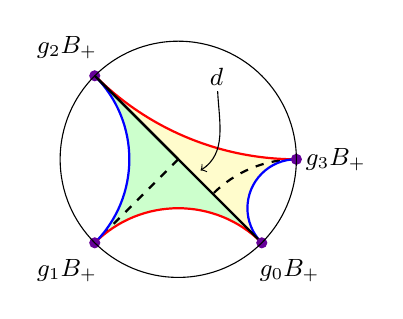
\begin{tikzpicture}
    \tikzset{font=\small}
    \begin{scope}[shift={(0,0)}]

      \fill[thick, even odd rule, fill=yellow!20!white]
            (135:1.5) to (315:1.5)
                      arc(225: 90:0.622)
                      arc(270:225:3.615)
        ;

      \fill[thick, even odd rule, fill=green!20!white]
            (315:1.5) to (135:1.5)
                      arc(405:315:1.5        )
                      arc(135: 45:1.5        )
        ;

      \begin{scope}
        \clip (0,0) circle (1.501);
        \draw[thick, dashed, black] (0,0) -- (225:1.5);
        \draw[thick, dashed, black] (  0:1.5) arc(90:135:1.5);
      \end{scope}

      \draw[thick, red ] (315:1.5) arc( 45:135:1.5);
      \draw[thick, blue] (225:1.5) arc(315:405:1.5);

      \draw[thick, red ] (  0:1.5) arc(270:225:3.615);
      \draw[thick, blue] (315:1.5) arc(225: 90:0.622);

      \draw[thick, black] (315:1.5) -- (135:1.5);

      \node at (  0:2.0) {$g_3 B_{+}$};
      \node at (135:2.0) {$g_2 B_{+}$};
      \node at (225:2.0) {$g_1 B_{+}$};
      \node at (315:2.0) {$g_0 B_{+}$};

      \node[circle, fill=red!40!blue, inner sep=0.5mm] at (  0:1.5) {};
      \node[circle, fill=red!40!blue, inner sep=0.5mm] at (135:1.5) {};
      \node[circle, fill=red!40!blue, inner sep=0.5mm] at (225:1.5) {};
      \node[circle, fill=red!40!blue, inner sep=0.5mm] at (315:1.5) {};

      \draw (0,0) circle (1.5);
      \draw[thick, black] (315:0.) -- (135:1.5);
      %\draw[thick, black] (315:0.4) -- ++( 45:0.1);

      \node (a02) at ( 65:1.15) {$d$};
      \draw[->] ( 60:1.00) to[bend right, out= 15, in=135] ($ (315:0.3) + ( 45:0.1) $);
    \end{scope}
  \end{tikzpicture}
\end{document}
